\section{Fremgangsmetode}

Der blev fra Linak's side foreslået at bruge kredsen BQ76920 til udvilking af den integrerede version, og da den havde de funktioner der skulle bruges (balancering, FET kontrol, temperatursensor, strøm- og spændingsmåling), var næste skridt at finde en microcontroller der kunne styre kredsen. Derefter blev softwaren udviklet, og de tilhørende komponenter dimensioneret. \\

Der er også tilføjet et spændingsnet som beskrevet i afsnit \ref{afs:voltagenet}, da den integrerede kreds kun kan levere omkring $20\milli\ampere$. Her er der behov for mere strøm da et display ønskes tilkoblet, og spændingsnettet kan levere $250\milli\ampere$. \\

Strømmålingen og balanceringskredsløbet vil ikke blive beskrevet her, da princippet er det samme som i henholdsvis afsnit \ref{afs:current_meas} og afsnit \ref{afs:balancing}. Transistorerne til balancering sidder internt i kredsen. 
\section{Valg af microcontroller}\label{afs:valg_af_uc}
Der blev besluttet at bruge microcontrolleren LPC804 til denne BMS. Den blev valgt af flere årsager:

\begin{itemize}[noitemsep]
	\item Lavt strømforbrug i deep sleep.
	\item ADC i 12-bits opløsning.
	\item De ønskede kommunikationsprotokoller er tilgængelige. ($I^2C$, $UART$)
	\item Microcontrolleren er NXP's billigere serie.
	\item Fås i både relativt små pakker samt store pakker.
	\item Evaluationboard er tilgængeligt.
\end{itemize}

Evaluationsboardet ved navn UM40001UL bliver brugt til udvikling af software. Dette board har onboard CMSIS-DAP som er en debugger, således det ikke er nødvendigt med en ekstern debugger. 

\section{Batteriovervågningskreds}\label{afs:bms_ic_desc}
Den integrerede kreds der er valgt klarer nærmest alle opgaver. Den står for overvågning af cellespændinger, balancering, styring af MOSFET's (charge og discharge), mulighed for ekstra temperaturmåling samt coloumb counting (strømmåling). \\

\begin{figure}[h]
	\centering
	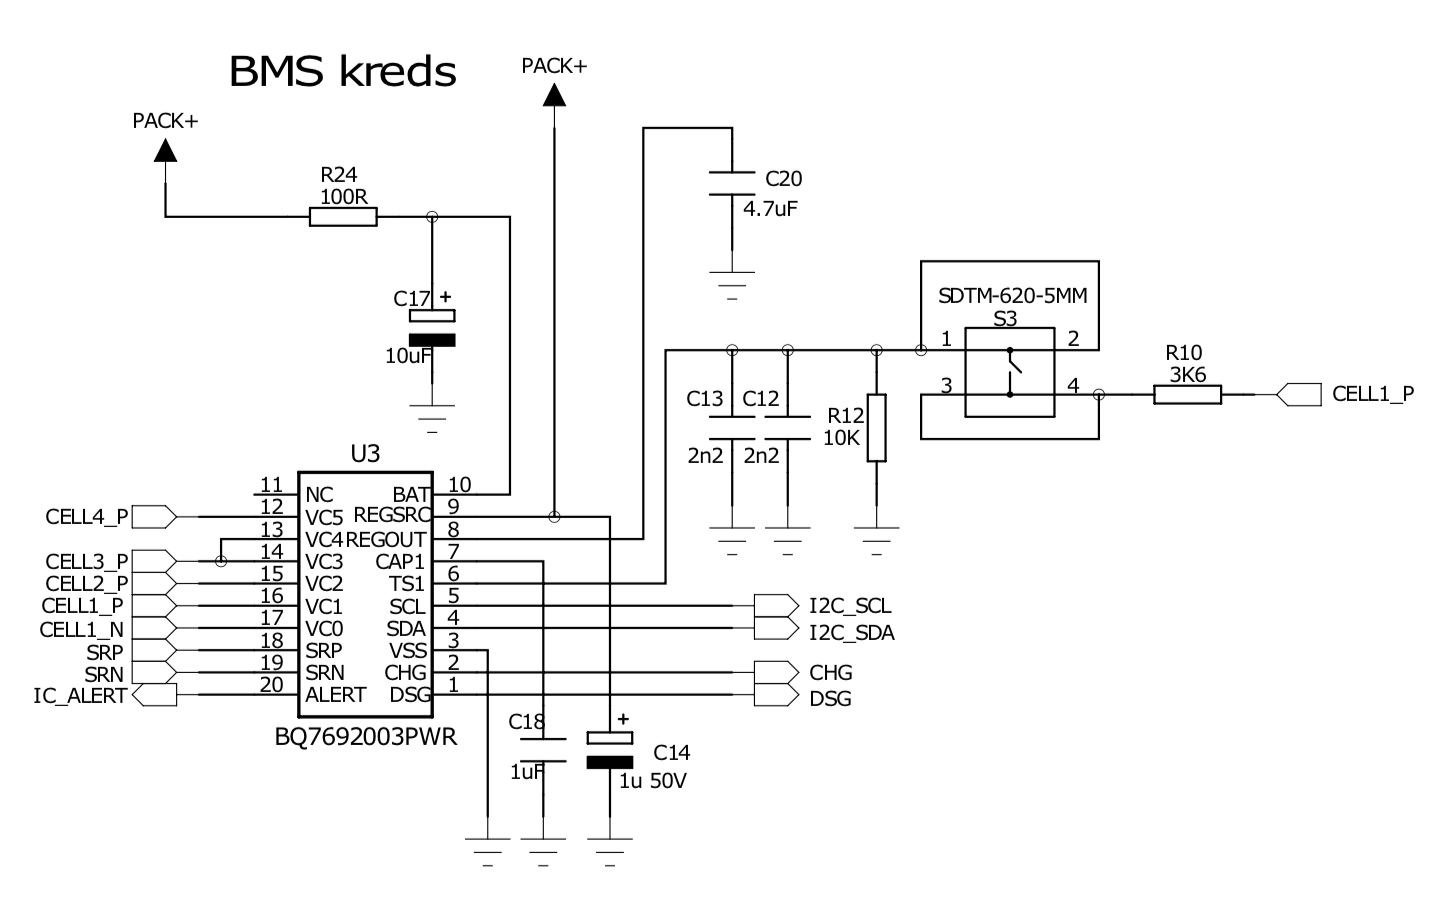
\includegraphics[width=15cm]{billeder/bms_ic_sch.png}
	\caption{Schematics for batteriovervågningskreds}
	\label{fig:temp_sensor}
\end{figure}

Da kredsen fungerer vha. kommunikation over I2C, sættes den først og fremmest til I2C bus'en. SDA er datalinjen og SCL er clock linjen. Tilslutningen ses på figur \ref{fig:temp_sensor}.

\subsection{ALERT kredsløb}
Kredsen har et ALERT ben som kan rapportere om at der er eventuelle status- eller fejlmeddelelser tilgængelige, men da kredsen har $2.5\volt$ logik på dette ben, er der indsat et kredsløb til at "konvertere" \space dette til $3.3\volt$ logik. Dette er realiseret med 2 npn-transistorer som ses på figur \ref{fig:bq_npn_conv}.

\begin{figure}[h]
	\centering
	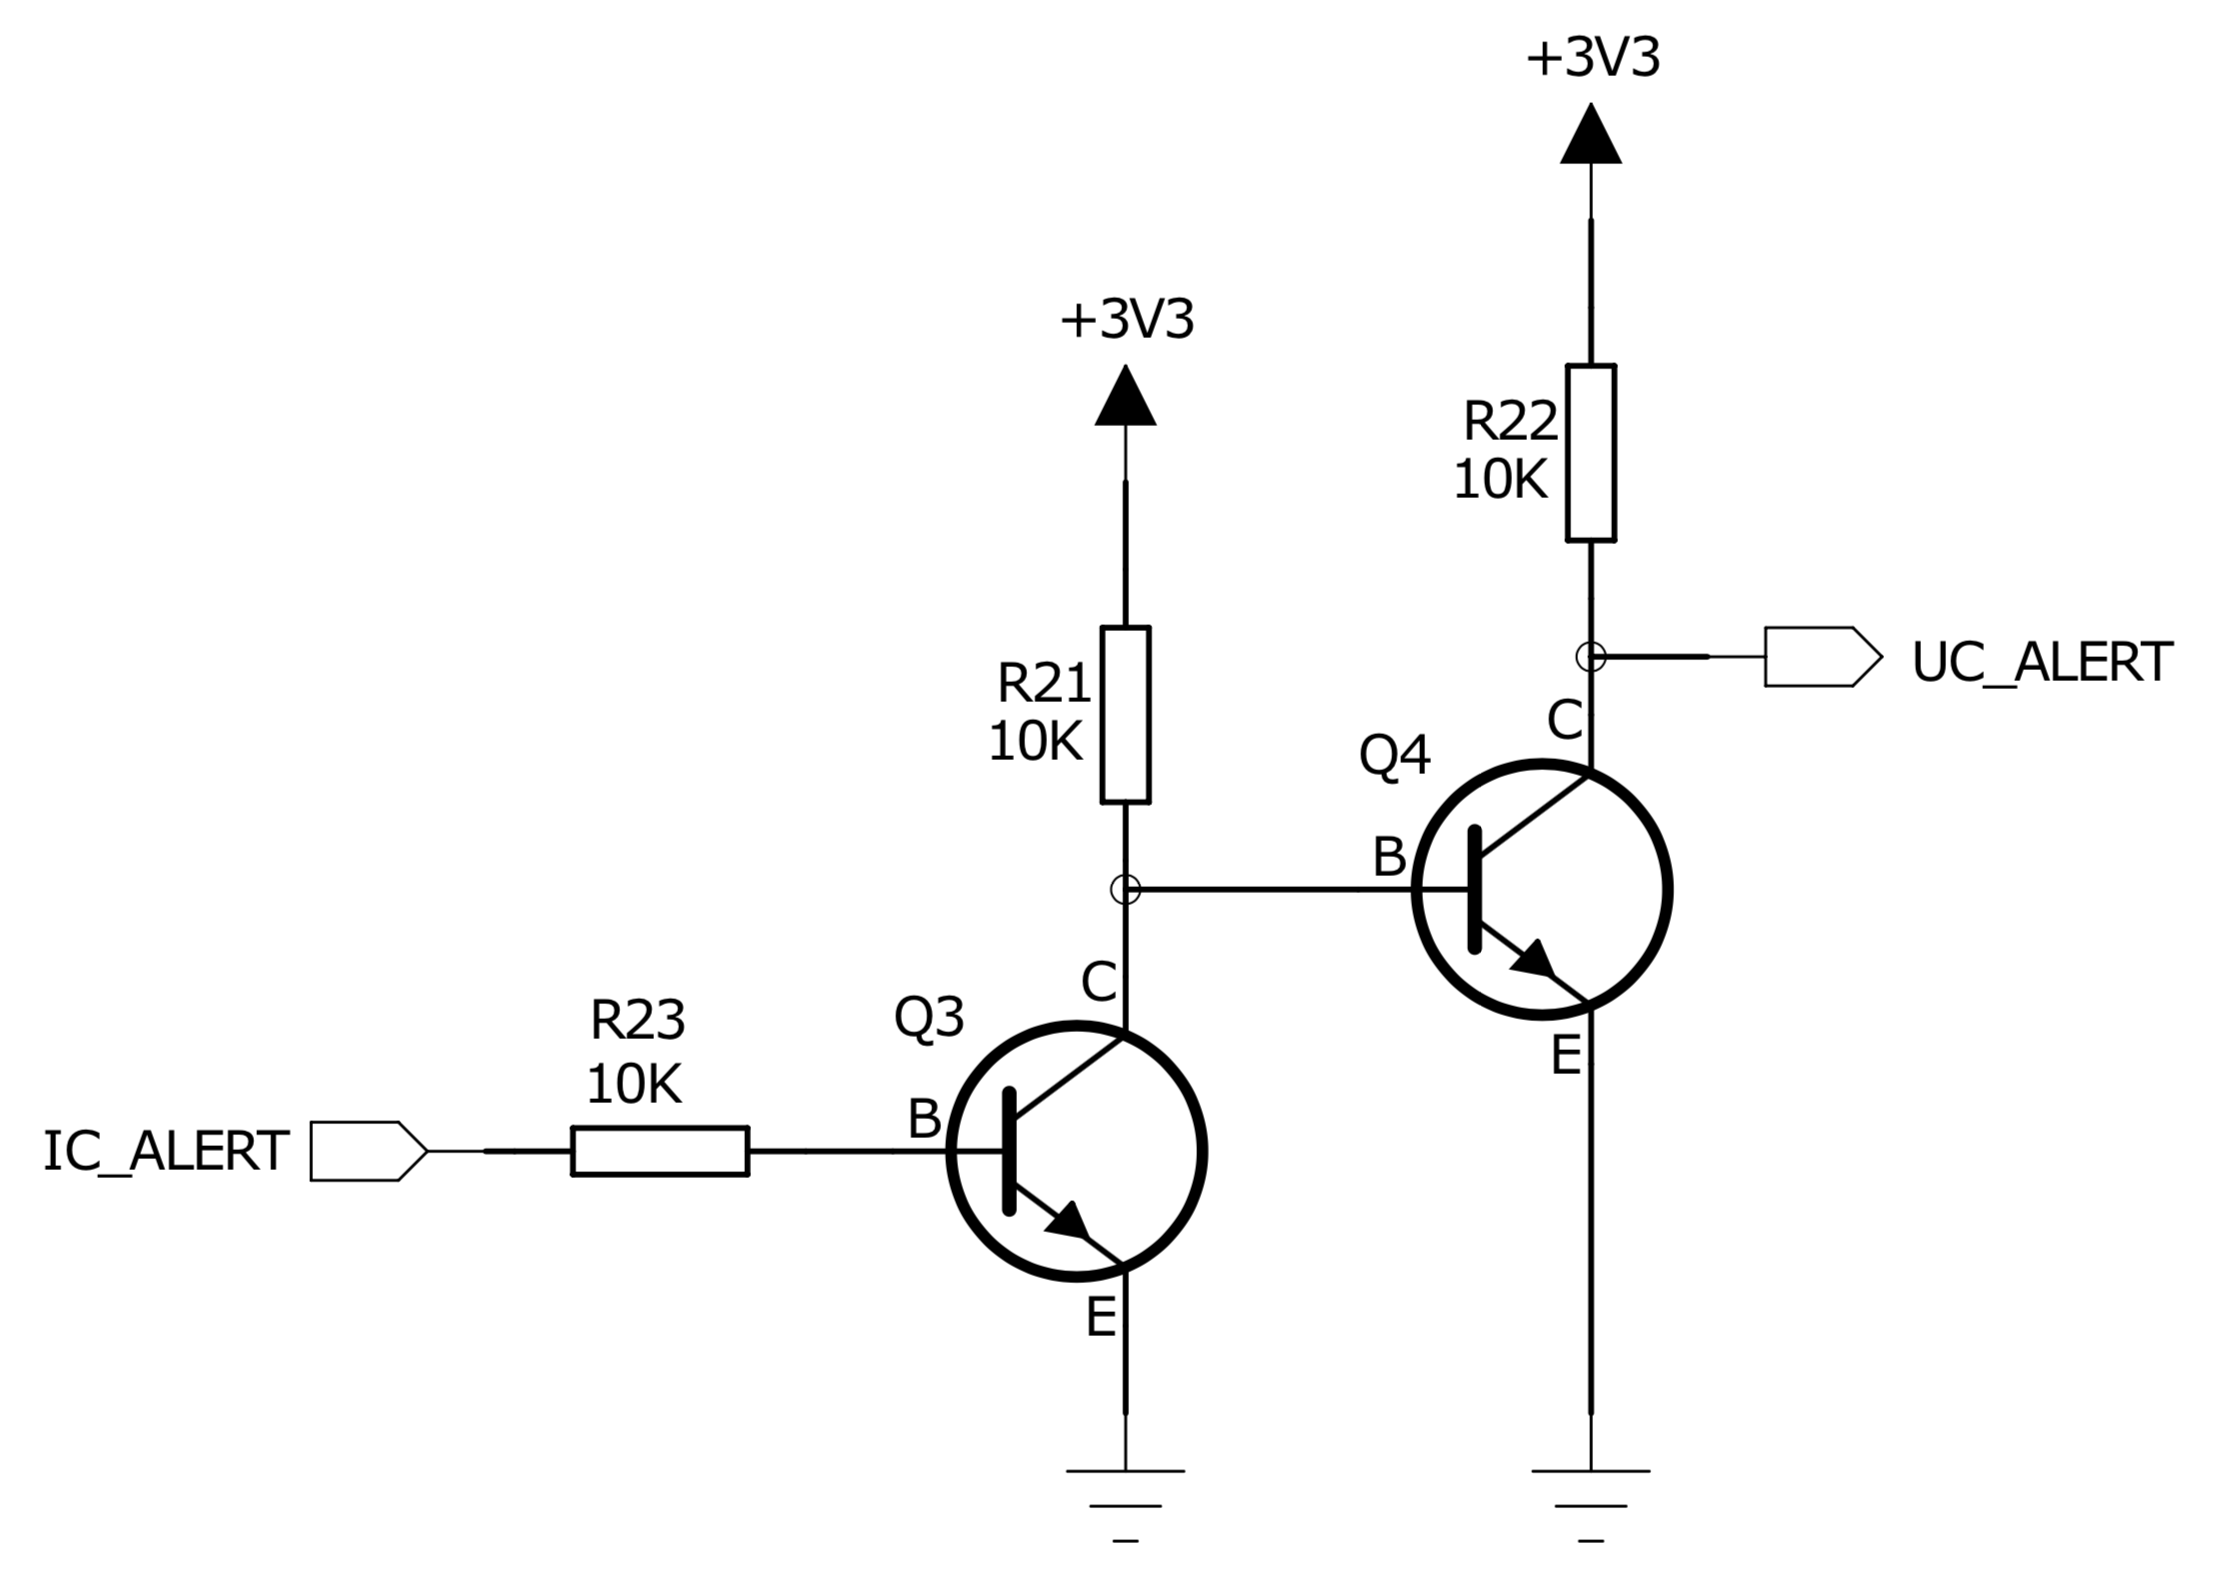
\includegraphics[width=10cm]{billeder/bq_npn_conv.png}
	\caption{Transistorkredsen til konvertering af 2.5V til 3.3V logik}
	\label{fig:bq_npn_conv}
\end{figure}

\subsection{MOSFET driver}
For at styre op- og afladnings MOSFET'erne, har BQ76920 indbygget MOSFET driver på CHG og DSG benene. Disse ben er internt drevet højt til $12\volt$ når de er slået til. Når slået fra, har DSG en hurtig pull-down til stel, mens CHG bruger en høj-impedant pull-down. 

\begin{figure}[h]
	\centering
	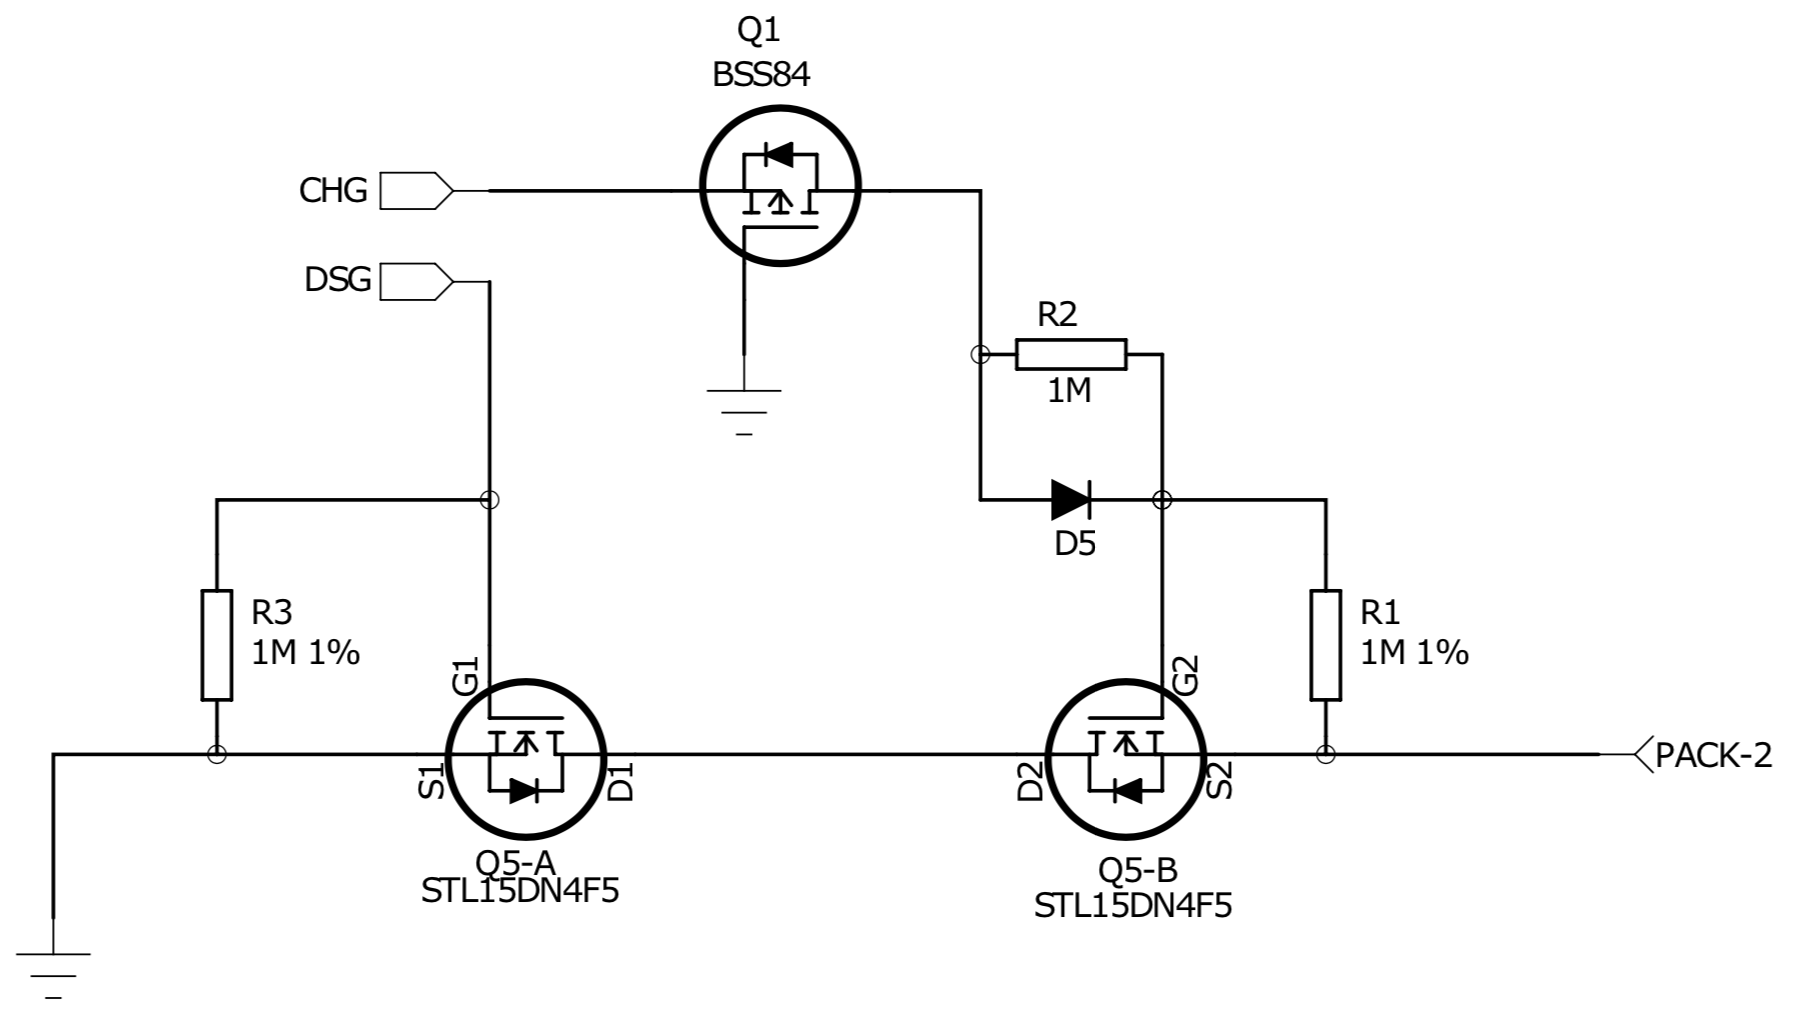
\includegraphics[width=11cm]{billeder/bq_fets.png}
	\caption{MOSFET's til styring af op- og afladning}
	\label{fig:bq_fets}
\end{figure}

Q5-A styrer afladningen og Q5-B styrer opladningen. Som der ses på figur \ref{fig:bq_fets} er der indsat en p-kanal's MOSFET (Q1) for at holde kredsens CHG ben væk fra negative spændinger. Når CHG ikke er slået til og PACK-2 f.eks. bliver trukket under stel, vil det ikke blive set af CHG benet da Q5-A ikke tænder. Q1 sørger også for at R2 kan holde Q5-B slukket, siden alle spændinger under denne FET kan "følge" \space PACK-2 hvis den går under stel. \\

Dioden (D5) sørger for at CHG kan trække Q5-B's gate høj. Modstanden i parallel (R2), får spændingen til at falde når PACK-2 er trukket høj, samtidig med den begrænser strømmen der går ind i CHG benet. Modstanden R1 holder Q5-B slukket når CHG er slukket.\footnote{Se datablad for BQ76920 på side 28; \url{http://www.ti.com/lit/ds/symlink/bq76920.pdf}}
\sbf{Tjek det stykke her...}

\section{Temperatursensor} \label{sec:temperatur}
Som endnu en sikkerhedsforanstaltning bruges en temperatursensor til at overvåge temperaturen i batteripakken. Her blev der besluttet at bruge en I2C temperatursensor, da opsætning ville være nemt siden I2C allerede skulle benyttes. Den specifikke del hedder LM75BIM-3/NOPB. Denne model blev valgt da den var tilgængelig på evaluation-boardet af microcontrolleren som blev brugt under udvikling. Derfor kunne udviklingen af software ske før hardware delen var helt færdig, og dermed fremskynde processen. \\ 

Brug af denne sensor giver også frihed til placering. Den bliver på denne BMS placeret på PCB'et med alle andre komponenter, da det ønskes at måle ambient temperatur for hele pakken, men kan evt. sættes på sit eget print tættere på cellerne for at få hver celles præcise temperatur. 

\subsection{Tilslutning af sensor}
Siden sensoren benytter $I^2C$, er den relativt nemt at tilslutte rent hardware mæssigt. SCL og SDA sættes til $I^2C$ bus'en på microcontrolleren, og OS benet sættes til et vilkårligt GPIO ben på microcontrolleren. A0, A1 og A2 forbindes alle til stel, da dette giver en 7-bits $I^2C$ adresse på 0x48, som ikke interfererer med andre adresser på bussen. \\

\begin{figure}[h]
	\centering
	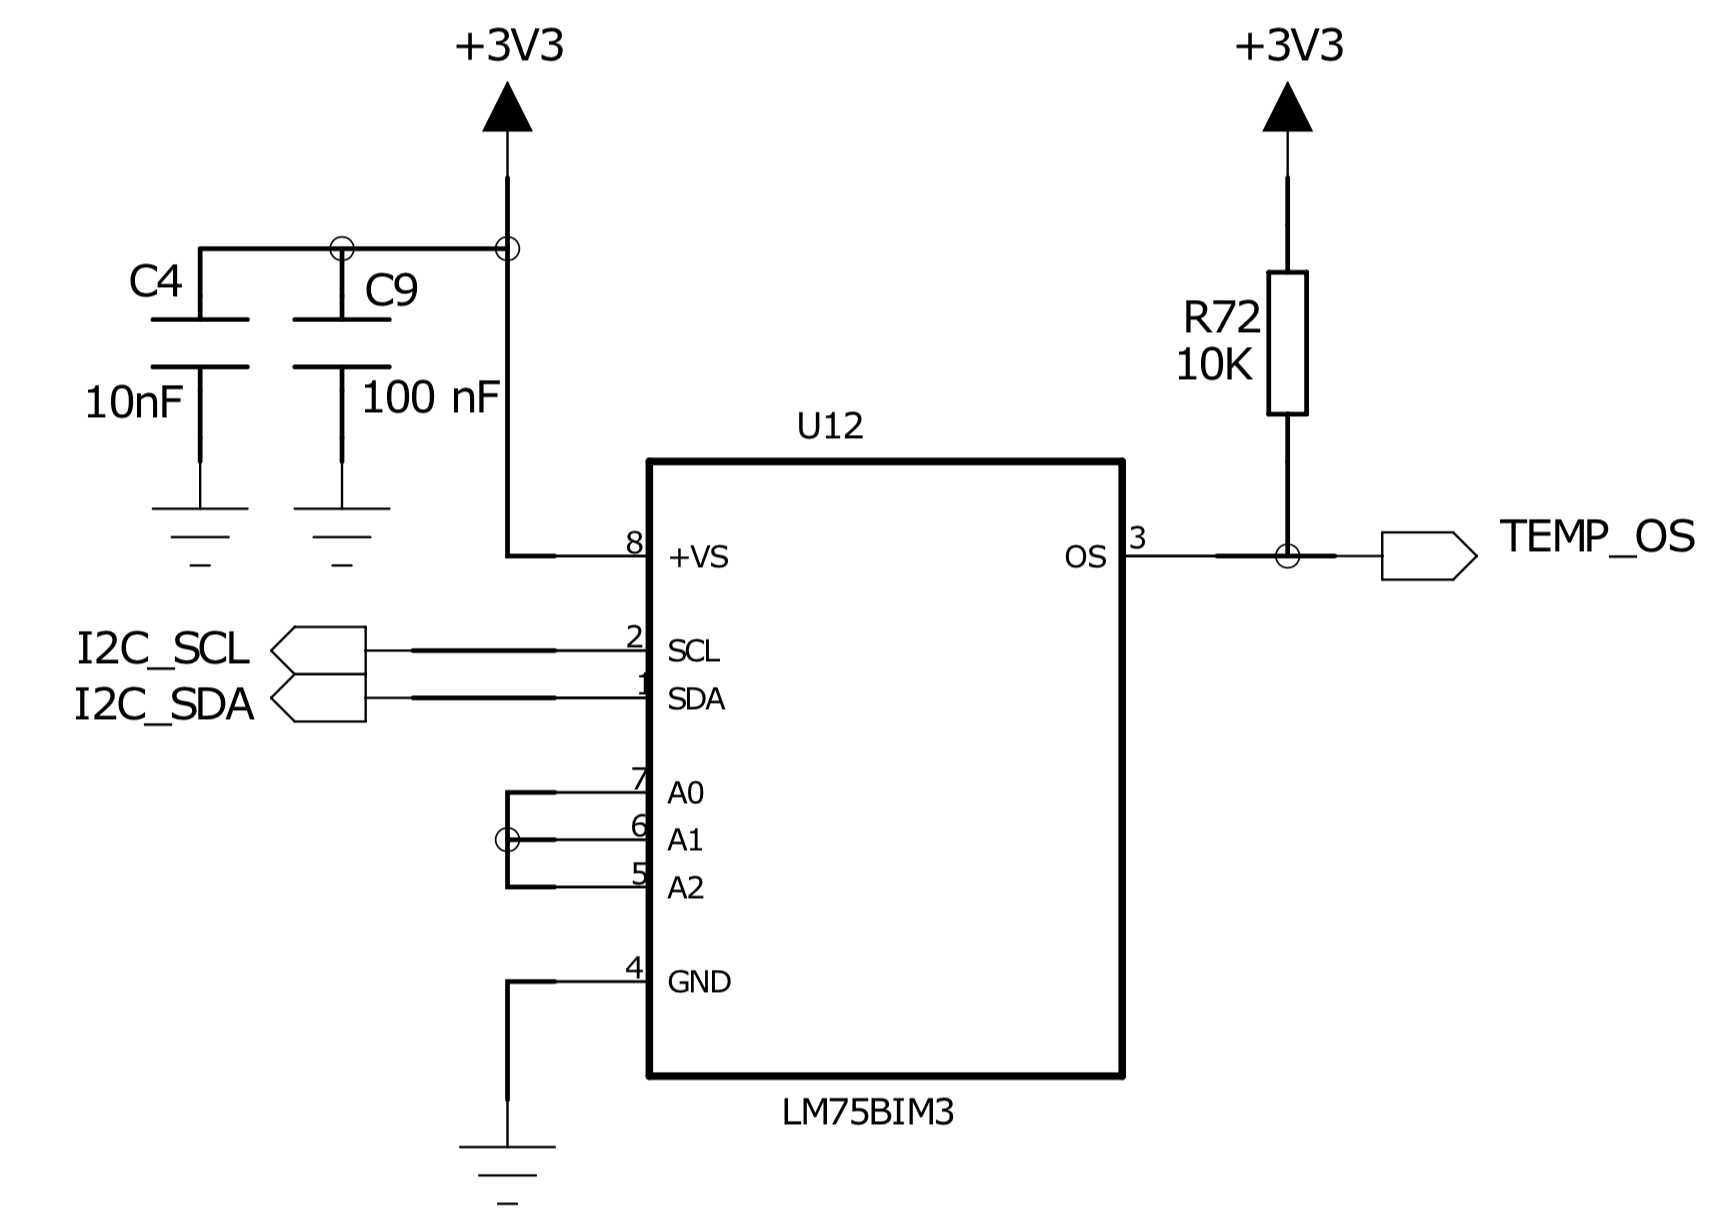
\includegraphics[width=11cm]{billeder/temp_sensor_sch.png}
	\caption{Schematics for temperatursensor}
	\label{fig:temp_sensor}
\end{figure}
\sbf{Photoshop billede så der er stel på A0-A2}

Dette ben (OS) er til eventuelle status meddelelser fra sensoren. Benet bliver ikke brugt i dette system, men er stadig tilføjet for eventuelt fremtidigt brug. Implementering af sensoren i software forklares i kapitel \ref{kap:softwareudvikling}.

\section{Udvikling og realisering af PCB}
For at skabe stabilitet til microcontolleren og systemet som helhed, og for at komprimere elektronikken er der valgt at designe et PCB. Det færdige PCB kan ses på figur \ref{fig:PCB_IC} og \ref{fig:PCB_IC_bagside}.

\begin{figure}[h]
	\centering
	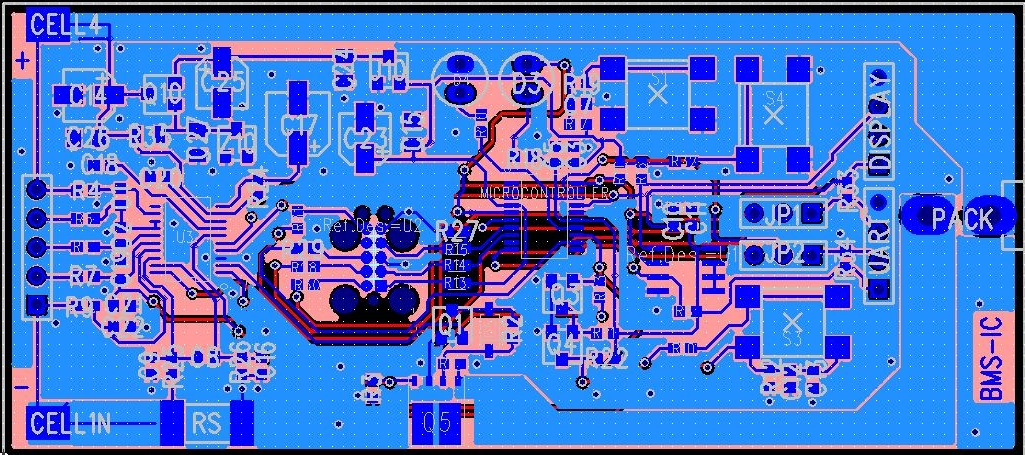
\includegraphics[width=15cm]{billeder/IC_1.jpg}
	\caption{Forsiden af PCB layout af BMS med batteriovervågningskreds.}
	\label{fig:PCB_IC}
\end{figure}

\begin{figure}[h]
	\centering
	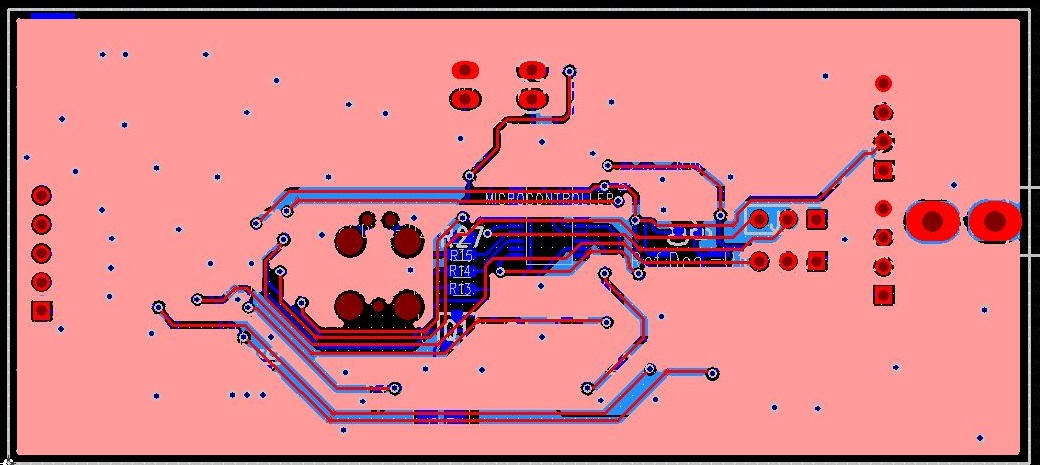
\includegraphics[width=15cm]{billeder/IC_2.jpg}
	\caption{Bagsiden af PCB layout af BMS med batteriovervågningskreds.}
	\label{fig:PCB_IC_bagside}
\end{figure}

Cellerne forbindes på venstre side af printet, hvor den enkelte celle er forbundet til et balanceringsben. Udgangsterminalen er placeret i højre side, hvor e

Banetykkelse
Balancering og connectors
Programmerings stik
Ind og udgange
